\documentclass[11pt,a4paper]{article}
\usepackage[utf8]{inputenc}
\usepackage{amsmath, mathtools}
\usepackage{amsfonts, dsfont}
\usepackage{amssymb}
\usepackage{graphicx}
\usepackage{empheq}
\usepackage{bm}
\usepackage[round, sort]{natbib}
\usepackage{tikz}
\usepackage{mathtools}  
%\mathtoolsset{showonlyrefs}  
\usetikzlibrary{shapes,backgrounds,arrows,automata,snakes,shadows,positioning, mindmap}

%%%%% Commands
\newcommand{\argmin}{\arg\!\min}
\newcommand{\argmax}{\arg\!\max}
\newcommand*\widefbox[1]{\fbox{\hspace{3em}#1\hspace{3em}}}
\newcommand*\lesswidefbox[1]{\fbox{\hspace{2em}#1\hspace{2em}}}
\newcommand{\entr}{\mathcal{H}}
\newcommand{\betabf}{\boldsymbol{\beta}}
\newcommand{\thetabf}{\boldsymbol{\theta}}
\newcommand{\mubf}{\boldsymbol{\mu}}
\newcommand{\Omegabf}{\boldsymbol{\Omega}}
\newcommand{\Sigmabf}{\boldsymbol{\Sigma}}
\newcommand{\zerobf}{\boldsymbol{0}}
\newcommand{\Xbf}{\boldsymbol{X}}
\newcommand{\xbf}{\boldsymbol{x}}
\newcommand{\Ybf}{\boldsymbol{Y}}
\newcommand{\Zbf}{\boldsymbol{Z}}
\newcommand{\Wbf}{\boldsymbol{W}}
\newcommand{\Ubf}{\boldsymbol{U}}
\newcommand{\Sbf}{\boldsymbol{S}}
\newcommand{\mbf}{\boldsymbol{m}}
\newcommand\Ncal{\mathcal{N}}
\newcommand\Pcal{\mathcal{P}}
\newcommand\Tcal{\mathcal{T}} 
\newcommand{\Esp}{\mathds{E}}
\newcommand{\bound}{\mathcal{J}}
\newcommand{\had}{\boldsymbol{\cdot}}

 %%%%%%% TIKZ
 \newcommand{\edgeunit}{1.5}
\providecommand\given{} % is redefined in \Set
\newcommand\SetSymbol[1][]{\nonscript\:#1\vert\nonscript\:}
%\usepackage[mathcal]{eucal}
\usepackage[left=2cm,right=2cm,top=2cm,bottom=2cm]{geometry}
\tikzset{%
    observed/.style={%
    scale=0.9,rectangle,draw=white,transform shape,fill=white,font=\Large}
}
\tikzset{%
    basic/.style={%
    scale=0.9,circle,draw=black,transform shape,fill=white,font=\small}
}


\setlength\parindent{0pt}
 \setcounter{tocdepth}{2}
\title{Reconstruction of a missing actor from count data using network inference}

\begin{document}

\maketitle
\vspace{3cm}


\section{Model}

$$\left\{\begin{array}{rl}
T & \sim\prod_{jk \in T} \beta_{jk}/B \\\\
\Ubf |T& \sim\mathcal{N}(0,R_T)\\\\
\Ybf|\Zbf&\sim\mathcal{P}( \exp( \Xbf\theta^\intercal + \Ubf\sigma^\intercal) )
\end{array} \right.$$

\paragraph{Dimensions:}
The model is build on matrices $\Ybf$ and $\Zbf$ with the following dimensions:\\
$\Ybf$: $n\times p$\\
$\Ubf_O$: $n\times p$\\
$\Ubf_H$: $n\times r$


\paragraph{Underlying dependencies:} This diagram is the graphical model behind the model, it describes the variables direct denpendencies and how data is simulated. Here, a tree $T$ is first drawn, which controls the dependency structure of parameters $\Ubf = (\Ubf_O,\Ubf_H)$. Count data $\Ybf$ is drawn from a distribution depending only on observed parameters $\Ubf_O$.
\begin{center}
	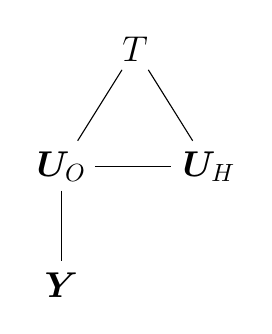
\begin{tikzpicture}	
      \tikzstyle{every edge}=[-,>=stealth',shorten >=1pt,auto,thin,draw]
		\node[observed] (A1) at (0.625*\edgeunit, 2*\edgeunit) {$T$};
		\node[observed] (A2) at (0*\edgeunit, 1*\edgeunit) {$\Ubf_O$};
		\node[observed] (A3) at (1.25*\edgeunit, 1*\edgeunit) {$\Ubf_H$};
		\node[observed] (A4) at (0*\edgeunit, 0*\edgeunit) {$\Ybf$};
		\path (A1) edge [] (A2)
        (A1) edge [] (A3)
        (A2) edge [] (A3)
        (A2) edge [] (A4);
	\end{tikzpicture}
\end{center}

\subsection{Distributions}
\label{distrib}
 
The complete vector of underlying parameters $\Ubf$ follows a mixture of normalized Gaussian distributions on the space of all existing spanning trees.
\begin{align*}
(\Ubf_O,\Ubf_H) &\sim \sum_{T \in \mathcal{T}} p(T) \mathcal{N}(0,R_T) \\
\end{align*}

 
Conditionally on the dependency structure $T$, $\Ubf$ is a centered Gaussian variable, with covariance matrix $R_T$ defined by block. As latent vectors are normalized, $R_T$ is a correlation matrix, and we define $\Upsilon$ its inverse. We obtain the following distributions:
\begin{align*}
(\Ubf_O,\Ubf_H)|T & \sim\mathcal{N}(0,R_T)\\
\Ubf_O|T & \sim\mathcal{N}(0,\Upsilon_{Tm}^{-1})
\end{align*}
 

Where  $ \Upsilon_{Tm} $ is the Schur's complement of $R_{TO}$: $\Upsilon_{Tm}=R_{TO}^{-1} =  \Upsilon_{TO} - \Upsilon_{TOH}\Upsilon_{TH}^{-1}\Upsilon_{THO}$. 

\subsection{Assumptions}
\paragraph{Assumption A:} The missing latent variables are not connected with each other. The $H$ bloc of $\Upsilon_T$ should thus be diagonal.

\paragraph{Assumption B:} To reduce the number of parameters, we assume that precision matrices which are faithful to different trees  only differ in the position of their zero entries, meaning that any trees sharing  an edge will also share the same value in their precision matrix. Let's define $\Upsilon$ such as $$\forall T_a \in \{T \in\mathcal{T} / kl \in T \}, \Upsilon_{T_a}[k,l] =  \Upsilon_ [k,l].$$

 Let's also define $I_T$ the binary matrix with diagonal one indicating the  edges presence in tree $T$ : $I_T=(\mathds{1}_{kl \in T} + \mathds{1}_{k=l})_{kl}$. Then we can write :
$$\forall T\in \mathcal{T}, \;\;\; \Upsilon_T = I_T \had \Upsilon $$
where '$\had$' denotes the Hadamard product. We obtain the following for $\Upsilon_T$, where the diagonal does not depend on $T$:
\[
 \Upsilon_T=
  \left( {\begin{array}{cc}
 (I_T \had \Upsilon)_O &  (I_T \had \Upsilon)_{OH}\\\\
 (I_T \had \Upsilon)_{HO} &   \Upsilon_H 
  \end{array} } \right) \]\\
 
 \section{Variational EM inference}
\subsection{Approximation of the likelihood}
\paragraph{Joint likelihood:}
The graphical model gives the following writing of the joint likelihood:
\begin{align*}
p(\Ybf,\Ubf,T)& = p(T) \: p(\Ubf|T) \: p(\Ybf|\Ubf) \\
&= p(T)\: p(\Ubf_O,\Ubf_H|T) \: p(\Ybf|\Ubf_O,\Ubf_H) \\
&= p(T) \: p(\Ubf_O|T) \: p(\Ubf_H | \Ubf_O,T)  \: p(\Ybf|\Ubf_O)
\end{align*} 


\paragraph{Variational approximation:}

Here $p(T,\Ubf \mid \Ybf)$ is untractable. We adopt a variational approximation aiming to maximise a lower bound of the log-likelihood of observed data $\log p(\Ybf)$, namely  
\begin{align*}
    \mathcal{J}(\Ybf; g,h)
    & = \log p(\Ybf) - KL\left[q(T,\Ubf) \mid\mid p(T,\Ubf \mid \Ybf)\right]
\end{align*}
Where KL is the Küllback-Leibler divergence. The approximation we adopt relies on factorizing $q$ in the product of two distributions $h$ and $g$ relating respectively to $\Ubf$  and $T$: 
$$p(T,\Ubf \mid\Ybf) \approx  q(\Ubf,T) = g(T)\:h(\Ubf).$$

 A consequence of this hypothesis is the contributions of   $\Esp_h[\log p(\Ubf\mid T)]$ and $\log p(T)$ --~only terms involving $T$ in the lower bound~-- writing as sums on the edges. As distribution   $g$ minimizes the KL divergence, it has to factorizes on the edges as well and hence:
$ g(T) = \left(\prod_{kl} \widetilde{\beta}_{kl} \right) / \widetilde{B}$. 

Moreover, it follows from the independence of the samples that $h$ is a product law: $ h(\Zbf) = \prod_i h_i(\Zbf_i)$.
Our variational approximation consists in assuming that each of its components is a multivariate Gaussian: $h(\Zbf_i) = \Ncal(\Zbf_i; \mbf_i, \Sbf_i)$, where $\Sbf_i$ is diagonal, meaning that $\Zbf_H$ and $\Zbf_O$ are independent under distribution $h$.  In the following we use the  $n\times (p+r)$ matrices $M$ and $S$ which compile respectively all vectors of means $\mbf_i$ and diagonals of variances $\Sbf_i$.


\paragraph{Lower bound:}
The lower bound of our model writes:
\begin{align*}
\mathcal{J}(\Ybf; g,h)&=\log p(\Ybf) - KL\left[g(T) h(\Ubf) \middle\vert\middle\vert\ p(T,\Ubf | \Ybf)\right]\\
&= \log p(\Ybf) - \Esp_{gh}[\log( g(T) h(\Ubf)) - \log p(\Ubf,T\mid \Ybf) ]\\
&= \log p(\Ybf) - \Esp_{gh}[\log g(T) + \log h(\Ubf) ] + \Esp_{gh}[\log p(\Ybf,\Ubf,T)] - \Esp_{gh}[\log p(\Ybf)]\\
&= \Esp_{gh} [\log p(\Ybf,\Ubf,T)] + \entr[g(T)] + \entr[h(\Zbf)]
\end{align*}

\begin{equation}
\label{firstJ}
 \boxed{\mathcal{J}(\Ybf; g,h) = \Esp_{gh} [\log (p_\beta(T)p_{\Upsilon}(\Ubf\mid T)p_{\theta, \sigma}(\Ybf\mid \Ubf))] + \entr[g_{\widetilde{\beta}}(T)] + \entr[h_{M,S}(\Ubf)]}
\end{equation}
Thus the model's parameters are $\Phi = (\theta,\sigma,M,S,\widetilde{\beta}, \beta,  \Upsilon)$.

\subsection{PLNmodels: optimizing in $\theta$, $\sigma$, and $h(\Ubf_O)$:}
\citet{CMR18} compute the lower bound of a VEM for the original PLN model, that is where no missing actor is assume and the independance structure of the latent layer of parameters is not supposed to be faithful to a tree. This lower bound, denoted $\mathcal{J}_{PLN}$  and implemented  in the R package \texttt{PLNmodels}, can be used in our computation as well.

\subsubsection{Rewriting  $\mathcal{J}(\Ybf; g,h)$}
Let's first separate observed and unobserved latent variables:
\begin{align*}
\mathcal{J}(\Ybf; g,h)&= \Esp_{gh}[\log p(T)  p(\Ubf_H| \Ubf_O,T) p(\Ubf_O|T)p(\Ybf|\Ubf_O)] + \entr[g(T)] +\entr[h(\Ubf_H,\Ubf_O)]
\end{align*}

 $\Ubf_O$ and $\Ubf_H$ being independent under the $h$ distribution, we have:
\begin{align*}
\entr[h(\Ubf_H,\Ubf_O)] &=\entr[h(\Ubf_O)] +\entr[h(\Ubf_H)]
\end{align*}

Now using the hypothesis of independence of $g$ and $h$, we obtain quantities with separate dependencies:
\begin{align}
\mathcal{J}(\Ybf; g,h)&=  \Esp_{gh}[\log p(\Ubf_O | T)] +\Esp_h[\log p(\Ybf|\Ubf_O)]+\entr[h(\Ubf_O)]  \label{PLNlike}\\
& \;\; + \Esp_{gh}[\log p(\Ubf_H | \Ubf_O,T) ]+\Esp_g[\log p(T)] +\entr[g(T)]+\entr[h(\Ubf_H)] \label{new}
\end{align}

Using again the independence of $g$ and $h$ to separate the expectation, and the linearity of the trace operator, the first term of the lower bound writes as the following:
\begin{align*}
\Esp_{gh}[\log p(\Ubf_O|T)] &=  \Esp_{gh} \left[\frac{n}{2} \log |\Upsilon_{Tm}| - \frac{1}{2} \sum_i \Ubf_{Oi}\Upsilon_{Tm} \Ubf_{Oi}^\intercal  \right]\\
&= \frac{n}{2} \Esp_g [\log |\Upsilon_{Tm}|] - \frac{1}{2} \Esp_{gh}\left[Tr\left( \Ubf_O^\intercal \Ubf_O \Upsilon_{Tm}\right)\right]\\
 &=\frac{n}{2} \Esp_g [\log |\Upsilon_{Tm}|] - \frac{1}{2}  Tr\left(\Esp_h [\Ubf_O^\intercal \Ubf_O ]\; \Esp_g[\Upsilon_{Tm}]\right). 
\end{align*}
Now introducing the quantity  $\log |\Esp_g [\Upsilon_{Tm}]| $  in (\ref{PLNlike}) we obtain:
\begin{align*}
\Esp_{gh}[\log p(\Ubf_O | T)] +\Esp_h[\log p(\Ybf|\Ubf_O)]+ \entr[h(\Ubf_O)] & = \frac{n}{2} \log |\Esp_g [\Upsilon_{Tm}]| - \frac{1}{2}Tr\left(\Esp_h [\Ubf_O^\intercal \Ubf_O ]\; \Esp_g[\Upsilon_{Tm}]\right)+ \entr[h(\Ubf_O)]\\
& \;\;\; + \Esp_{h}[\log p(\Ybf|\Ubf_O)] +  \frac{n}{2}\left( \Esp_g[\log|\Upsilon_{Tm}|] - \log|\Esp_g [\Upsilon_{Tm}]|\right)
\end{align*}

Wtih $\Esp_g [\Upsilon_{Tm}]$ as a precision matrix for $\Ubf_O$, the lower bound $\mathcal{J}_{PLN}(\Esp_g [\Upsilon_{Tm}]^{-1})$ appears:
 $$\Esp_{gh}[\log p(\Ubf_O | T)] +\Esp_h[\log p(\Ybf|\Ubf_O)]+ \entr[h(\Ubf_O)] = \mathcal{J}_{PLN} (\Esp_g [\Upsilon_{Tm}]^{-1})- \frac{n}{2}\left( \Esp_g[\log|\Upsilon_{Tm}|] - \log|\Esp_g [\Upsilon_{Tm}]|\right)$$
 \subsubsection{Maximisation and correction of $\mathcal{J}(\Ybf; g,h)$}
As the last term do not depend either on $\theta$ or $h(\Zbf_O)$, we finally obtain that
 $$ \argmax_{\theta, h(\Ubf_O)} \big\{\Esp_{gh}[\log p(\Ubf_O | T)] +\Esp_h[\log p(\Ybf|\Ubf_O)]+ \entr[h(\Ubf_O)]\big\} = \argmax_{\theta, h(\Ubf_O)} \big\{ \mathcal{J}_{PLN}(\Esp_g [\Upsilon_{Tm}]^{-1})\big\}.$$


\subsection{VE step: optimizing in $g$ and $h(\Zbf_H)$}
The VE step minimizes the Küllback-Leibler divergence between the approximated and the aimed distributions :

$$  \argmin_{g,h(\Ubf_H)} KL\left(g(T)h(\Ubf) \mid\mid p(\Ubf,T|\Ybf)\right)$$

\begin{align*}
KL\left(g(T)h(\Ubf) \mid\mid  p(\Ubf,T|\Ybf)\right) &= \Esp_{gh}\left[\log g(T)h(\Ubf) - \log p(\Ubf,T\mid \Ybf) \right]\\
&= \Esp_{gh}\left[\log g(T)h(\Ubf) - \log p(\Ybf,\Ubf,T) + \log p(\Ybf)  \right]\\
&= \Esp_{gh}\left[\log g(T)+ \log h(\Ubf) - \log (p(T)p(\Ubf\mid T) p(\Ybf\mid \Ubf_O)) + \log p(\Ybf)  \right]\\
&= -\Esp_{gh}[\log p(\Ubf \mid T) ] - \Esp_g[\log p(T) - \log g(T)] - \entr[h(\Ubf)]\\
& \;\;\;\; -\Esp_h[\log p(\Ybf \mid \Ubf_O)] +\log p(\Ybf) 
\end{align*}
Distributions $p(\Ybf)$ and $p(\Ybf\mid \Ubf_O)$  do not depend on distributions $g$ and $h(\Ubf_H)$. Moreover, as $\Ubf_O$ and $\Ubf_H$ are independant under the $h$ distribution, $\entr[h(\Ubf)] = \entr[h(\Ubf_O)]+ \entr[h(\Ubf_H)]$ and  $\entr[h(\Ubf_O)]$ is already optimized. We obtain:
 
\begin{empheq}[box=\widefbox]{align*}
\argmin_{g,h(\Ubf_H)} KL  &=\argmin_{g,h(\Ubf_H)} \Big\{ -\Esp_{gh}[\log p(\Ubf \mid T) ] - \Esp_g[\log p(T) - \log g(T)] -\entr[h(\Ubf_H)] \Big\}
\end{empheq}
 
 During the minimization, we will use the optimized distribution $h(\Ubf_O)^* = \prod_i^n \mathcal{N}(\widetilde{\mbf}_{Oi}, \widetilde{S}_{Oi})$, its parameters being gathered in $n\times p$ matrices $\widetilde{M}_O$ and $\widetilde{S}_O$.
 
 \subsubsection{Details of  $\Esp_{gh}[\log p(\Ubf \mid T) ]$} 
 $$\log p(\Ubf \mid T) = -\frac{n}{2} \log |R_T| - \frac{1}{2} Tr(\Upsilon_T \times \Ubf^\intercal \Ubf) $$
 Taking the expectation, and by independence of $g$ and $h$:
 $$\Esp_{gh} [\log p(\Ubf \mid T)] = \frac{n}{2} \Esp_{gh} [\log | \Upsilon_T|] - \frac{1}{2} Tr(\Esp_g[\Upsilon_T] \Esp_h[\boldsymbol{U}^\intercal \boldsymbol{U}])$$
 
From the definition of the $h$ distribution: $$ \Esp_h[\Ubf^\intercal \Ubf] = M^\intercal M + S = SSD$$
 Where SSD is the sum of squared deviances and is a suffiencient statistic of the distribution. As latent vectors are normalized, SSD has diagonal 1.
 
\paragraph{Expectation of the log-determinant of $\Upsilon_T$\\}
Thanks to $\Upsilon_T$ being tree-structured, its determinant factorizes on the edges of $T$ as follows:
\begin{align*}
|\Upsilon_T| &=\frac{ \prod_{kl \in T} |R_{T[kl]}|}{\prod_k (r_{Tkk})^{deg(k)-1}} =  \prod_{kl \in T} (1-r_{Tkl}^2),
 \end{align*}
 which can be estimated using that $\forall kl \in T, r_{kl} = \frac{ssd_{kl}}{n}$,
 which gives $$\Esp_g[\log|\hat{\Upsilon}_T|]=\frac{1}{2}\sum_{kl} P_{kl}\log(1-\frac{ssd_{kl}^2}{n^2}).$$
\paragraph{Trace of expectations\\}
  \[ \Esp_g[\Upsilon_T]_{kl}  =  \Esp_g[I_T\had\Upsilon]_{kl} \left\{ 
\begin{array}{cc}
(P \had \Upsilon)_{kl} & k \neq l\\
\upsilon_{kk} & k = l
\end{array}
\right.
\]
Therefore we obtain $Tr(\Esp_g[\Upsilon_T] SSD) = \sum_{kl} P_{kl} \upsilon_{kl} ssd_{kl} + \sum_k \upsilon_{kk} $.\\

Finally, 
\begin{empheq}[box=\lesswidefbox]{align*}
\Esp_{gh} [\log p(\Ubf \mid T)] =  \frac{n}{4}\sum _{\substack{kl\\ k \neq l}} P_{kl} \log \Big(1-\frac{ssd_{kl}^2}{n^2}\Big) - \frac{1}{2}\sum_{\substack{kl\\ k \neq l}} P_{kl} \upsilon_{kl} ssd_{kl} - \frac{1}{2} \sum_{k} \upsilon_{kk} 
 \end{empheq}
\subsubsection{Details of $\Esp_g[\log g(T) - \log p(T)]$}
\begin{align*}
\log g(T) - \log p(T) &= \left(  \sum_{j<k} \mathds{1}\{jk \in T\} \log \widetilde{\beta}_{jk} - \log \widetilde{B}\right) - \left(  \sum_{j<k} \mathds{1}\{jk \in T\} \log {\beta}_{jk} - \log {B}\right)\\
&=\frac{1}{2}\sum_{jk} \mathds{1}\{jk \in T\} \log \frac{\widetilde{\beta}_{jk}}{{\beta}_{jk}} - \log \frac{\widetilde{B}}{B}
\end{align*}
$$\boxed{
\Esp_g[\log g(T) - \log p(T)] = \frac{1}{2}\sum_{jk}P_{jk} \left(\log \frac{\widetilde{\beta}_{jk}}{{\beta}_{jk}}\right) - \log \frac{\widetilde{B}}{B} }$$

 \subsubsection{Details of $\entr[h(\Ubf_H)]$}
 
 The entropy of the Gaussian multivariate vector $\Ubf_H$ mainly depends on its variance matrix $S_H$. By definition of $S_H$ we have:
 \begin{align*}
 \log |S_H| &= \log(\prod_{k=p+1}^{p+r} \sum_{i=1}^n S_{ik})
\end{align*}
which gives the following entropy:
\begin{align*}
\entr[h(\Ubf_H)]&= \frac{1}{2} \log |S_H| + \frac{nr}{2}(1+\log(2\pi))\\
 &=\frac{1}{2}\left[ \sum_{k=p+1}^{p+r} \log\left(\sum_{i=1}^n S_{ik}\right)+ nr(1+\log 2\pi )\right]
\end{align*}

\subsubsection{Final quantity to optimize:}
\begin{align*}
\argmin_{g,h(\Ubf_H)} KL  &=\argmin_{g,h(\Ubf_H)}  \Big\{-\Esp_{gh}[\log p(\Ubf \mid T) ] + \Esp_g[\log g(T) - \log p(T)-\entr[h(\Ubf_H)]\Big\}\\
&= \argmin_{g,h(\Ubf_H)}  \bigg\{- \frac{n}{4}\sum _{\substack{kl\\ k \neq l}} P_{kl} \log \Big(1-\frac{ssd_{kl}^2}{n^2}\Big) + \frac{1}{2}\sum_{\substack{kl\\ k \neq l}} P_{kl} \upsilon_{kl} ssd_{kl} + \frac{1}{2} \sum_{k} \upsilon_{kk} \\
& \;\;\;\; + \frac{1}{2}\sum_{\substack{kl\\ k\neq l}}P_{kl} \left(\log \frac{\widetilde{\beta}_{kl}}{{\beta}_{kl}}\right) - \log \frac{\widetilde{B}}{B} -\frac{1}{2}\sum_{k\in H} \log\left(\sum_i \widetilde{S}_{ik}\right) \bigg\}
\end{align*}
 
 
 \subsubsection{Update formulas for $\widetilde{\beta}$ and $M_H$ }

\paragraph{Edges weights under the $g$ distribution \\}
Let's isolate the terms referring to the edges in the expression to be minimized:
\begin{align*}
  \sum_{\substack{kl\\ k \neq l}} \frac{P_{kl}}{2}\Big(\log \widetilde{\beta}_{kl} - \log \beta_{kl} - \frac{n}{2} \log (1-\frac{ssd_{kl}^2}{n^2}) + \upsilon_{kl}\: ssd_{kl} \Big)   
\end{align*}

 
Equating the term $kl$ of the above sum to zero, we obtain:
 $$\log \widetilde{\beta}_{kl} = \log \beta_{kl} +  \frac{n}{2} \log  \left(1-\frac{ssd_{kl}^2}{n^2}\right) - \upsilon_{kl}\:ssd_{kl} $$
 
Which gives the following update formula for $\widetilde{\beta}_{kl}$:
 
  $$\boxed{\displaystyle \widetilde{\beta}_{kl} = \beta_{kl} \: \left(1-\frac{ssd_{kl}^2}{n^2}\right)^{n/2} \exp( -\upsilon_{kl}\: ssd_{kl} ) }$$


\paragraph{Means of the hidden part of the latent Gaussian vector under the $h$ distribution \\}
Means $M_H$ only appear in the $H$, $OH$ and $HO$ blocs of $SSD$. The derivative of KL with respect to mean $M_{ik}$ for the $i^\text{th}$ sample of species $k\in H$ writes:

\begin{align*}
\frac{\partial KL}{\partial M_{ik}} &=\frac{n}{2}\frac{\partial}{\partial M_{ik}}\Big(2\sum_{\substack{k \neq l\\
(k, l) \in H\times O}} P_{kl} \upsilon_{kl} (M^\intercal M)_{kl} + \sum_{k\in H} \upsilon_{kk} (M^\intercal M)_{kk}\Big)\\
&= n( \sum_{l \in O } M_{il} P_{kl}\upsilon_{kl} + M_{ik} \upsilon_{kk}) 
\end{align*}
\begin{align*}
\frac{\partial KL}{\partial M_{ik}}  = 0\iff M_{ik} &= -\frac{1}{\upsilon_{kk}} \sum_{l\in O} M_{il} (P\had\Upsilon)_{lk}\\
&=-\frac{M_{iO} (P\had\Upsilon)[O,H]}{\upsilon_{kk}}
\end{align*}

As $\Upsilon_H$ is diagonal, this  matricially comes down to
$$\boxed{ M_H = -M_O(P\had\Upsilon)_{OH} \Upsilon_H^{-1}}$$


\paragraph{Variances of the hidden part of the latent Gaussian vector under the $h$ distribution \\}
$S-H$ appears in the entropy of $h(\Zbf_H)$ and in the diagonal of $\Sigma$. 
\begin{align*}
\frac{\partial KL}{\partial S_{ik}} &= \frac{1}{2}  \frac{\partial KL}{\partial S_{ik}}  \Big(\sum_k \upsilon_{kk}(\sum_j S_{j k}) - \sum_k \log (\sum_jS_{j k})\Big)\\
&=\upsilon_{kk} - \frac{1}{S_{ik}}
\end{align*}
We obtain for $k\in H$ and all $i$:
$$\boxed{S_{ik} = 1/\upsilon_{kk}}$$

\subsubsection{Computing edge probabilities under $g$}
During computations, we need the edge probability under the $g$ distribution. This can be computed as the sum of probabilities of trees containing this edge:

\begin{align*}
\mathds{P}_g(kl \in T)  &= \sum_{\substack{T  \in \mathcal{T} \\ kl \in T }} g(T) =\frac{1}{\widetilde{B}} \sum_{\substack{T  \in \mathcal{T} \\ kl \in T }} \prod_{uv \in T} \widetilde{\beta}_{uv}
\end{align*}
where $\displaystyle \widetilde{B}= \sum_{T \in \mathcal{T} }\prod_{uv \in T}  \widetilde{\beta}_{uv}$.\\

 This is again a sum-product form, but on a special set of trees. This can be efficiently computed using a formula from \citet{kirshner} (Theorem 3), stated in the appendix.
 
 
 \subsection{M step: optimizing in $(\beta, \Upsilon)$}
 The M step aims at maximizing the lower bound in the parameters referring to original distributions for $T$ and $\Ubf|T$, therefore $\beta$ and $\Upsilon$. From Eq.(\ref{firstJ}) we obtain that: 
$$ \argmax_{\beta, \Upsilon} \mathcal{J}(\Ybf ; g,h) =\argmax_{\beta, \Upsilon} \left\{ \Esp_{gh} [\log (p_\beta(T)p_{\Upsilon_T}(\Ubf\mid T) ]\right\} $$

As distributions of VE step mimic original ones, computations are very similar. We get:
\begin{align*}
\log (p_\beta(T)p_{\Upsilon_T}(\Ubf\mid T))  &= \sum_{k<l} \mathds{1}\{kl \in T\} \log \beta_{kl} - \log B + \frac{n}{2}\log |\Upsilon_T| - \frac{1}{2}Tr(\Upsilon_T \Ubf^\intercal \Ubf)\\
\Esp_{gh} [\log (p_\beta(T)p_{\Upsilon_T}(\Ubf\mid T) ] &= \sum_{k<l} P_{kl} \log\beta_{kl} +\frac{n}{2} \Esp_g[\log |\Upsilon_T|] -\frac{1}{2} Tr(\Esp_g [\Upsilon_T] \; SSD)- \log B
\end{align*}

Reminding that $\Esp_g[\log |\Upsilon_{T}|]= \frac{1}{2}\sum _{kl} P_{kl}  \log \left(1-\frac{ssd_{kl}^2}{n^2}\right)$,  we obtain:
\begin{align*}
\Esp_{gh} [\log (p_\beta(T)p_{\Upsilon_T}(\Ubf\mid T) ] &=\frac{1}{2}\sum_{kl} P_{kl} \log  \beta_{kl} - \log B + \frac{n}{4} \sum_{kl} P_{kl} \log\left(1-\frac{ssd_{kl}^2}{n^2}\right)  - \frac{1}{2}Tr( (P \had \Upsilon) SSD)\\
&= \frac{n}{2}\left( \sum_k \log \omega_{kk}  + \frac{1}{2} \sum_{kl} P_{kl} \log \varphi_{kl} - \sum_{k} \omega_{kk} \sigma_{kk} - \sum_{kl} P_{kl} \omega_{kl} \sigma_{kl}\right)\\
& \;\; +\sum_{k<l} P_{kl} \log  \beta_{kl} - \log B 
\end{align*}
 
 $$\boxed{\Esp_{gh} [\log (p_\beta(T)p_{\Omega_T}(\Zbf\mid T) ]  =  \frac{n}{2} \sum_{kl} P_{kl} ( \frac{1}{2} \log \varphi_{kl} -\omega_{kl} \sigma_{kl} ) + \frac{n}{2} \sum_k (\log \omega_{kk} - \omega_{kk} \sigma_{kk}) +\sum_{k<l} P_{kl} \log  \beta_{kl} - \log B }$$
%%%%%%%%%%%%%% 
\newpage
\bibliographystyle{apsrev} %tested plainnat
\bibliography{bibi}
 \appendix
\section{Calcul du déterminant}
Dans la suite $\Sigma$ est fidèle à l'arbre $T$, et $\Sigma^{-1} = I_T\cdot \Omega$. D'après Lauritzen (5.12):
$$\frac{\omega_{\mu\Upsilon}^2}{\omega_{\mu\mu}\omega_{\Upsilon\Upsilon}} = c_{\mu\Upsilon}^2 = 1-\frac{|\Sigma|\;|\Sigma_{\setminus \{\mu\Upsilon\}}|}{|\Sigma_{\setminus\Upsilon}|\;|\Sigma_{\setminus \mu}|} $$

$\Sigma$ étant fidèle à un arbre, son déterminant se factorise simplement sur les arêtes en produit de leur corrélations, de telle sorte que :
\begin{align*}
    |\Sigma| &= \prod_k \sigma_{kk} \prod_{kl\in T} (1-\rho_{kl}^2)\\
    |\Sigma_{\setminus\Upsilon}| &= \prod_{k \neq \Upsilon} \sigma_{kk} \prod_{\substack{kl\in T \\ k \neq \Upsilon}} (1-\rho_{kl}^2)\\
    |\Sigma_{\setminus \{\mu\Upsilon\}}| &= \prod_{k\notin \{\mu, \Upsilon\}} \sigma_{kk} \prod_{\substack{kl\in T\\ (kl) \notin \{\mu, \Upsilon\}^2 }} (1-\rho_{kl}^2)
\end{align*}
Alors :
\begin{align*}
    \frac{|\Sigma|\;|\Sigma_{\setminus \{\mu\Upsilon\}}|}{|\Sigma_{\setminus\Upsilon}|\;|\Sigma_{\setminus \mu}|} &=\frac{\prod_k \sigma_{kk} \prod_{k\notin \{\mu, \Upsilon\}} \sigma_{kk}}{\prod_{k \neq \Upsilon} \sigma_{kk} \prod_{k \neq \mu} \sigma_{kk}} \times \frac{ \prod_{kl\in T} (1-\rho_{kl}^2)\prod_{\substack{kl\in T\\ (kl) \notin \{\mu, \Upsilon\}^2 }} (1-\rho_{kl}^2)}{\prod_{\substack{kl\in T \\ k \neq \Upsilon}} (1-\rho_{kl}^2)\prod_{\substack{kl\in T \\ k \neq \mu}} (1-\rho_{kl}^2)} \\
    &=\frac{(1-\rho_{\mu\Upsilon}^2)}{\prod_{\substack{kl\in T\\ (kl) \notin \{\mu, \Upsilon\}^2 }} (1-\rho_{kl}^2)} \times \prod_{\substack{kl\in T\\ (kl) \notin \{\mu, \Upsilon\}^2 }} (1-\rho_{kl}^2)\\
     &=1-\rho_{\mu\Upsilon}^2
\end{align*}
Finalement : 
$$\boxed{c_{\mu\Upsilon}^2 = \rho_{\mu\Upsilon}^2}$$

On peut alors écrire
$$ |\Sigma| = \prod_k \sigma_{kk} \prod_{kl \in T} (1-c_{kl}^2)$$
\end{document}